\chapter{Architecture and implementation of the Data Integration part}

As stated in the Requirements chapter, the Data Integration part must incrementally pull various REST APIs (data sources) in parallel. For each resource type in
in each data source, it must create an event flow. This event flow run through several data cleaning and data transformation steps that can
be asynchronous. Despite the asynchronous nature, it should ensure that the event flow remains in-order. In the end, event flows are pushed
into the Journal.

\section{Architecture}

\subsection{Puller actor system}

In order to pull periodic incremental pull of data sources, an Akka Actor system is defined. 

First, the system needs for each data source to receive a "top" message corresponding to the fact that a certain data source must be queried. We will use for this
Akka Quartz \footfullcite{bib:akkaquartz}, a cron-style scheduler that allows to define periodic sending of certain types of messages. An usual pull rate for a data source
is every 5 seconds, in order to create a near-realtime stream.
\\

These top messages will be received by a singleton actor named \verb|JobScheduler|. The purpose of the JobScheduler is to launch a child actor for each job (a job
corresponds to an incremental pull from a certain data source). Once the child actor has finished the incremental pull, it kills itself. Figure \ref{fig:archi_actor_dataintegration} illustrates this architecture.

\begin{figure}[h]
  \begin{center} 
    \makebox[\textwidth]{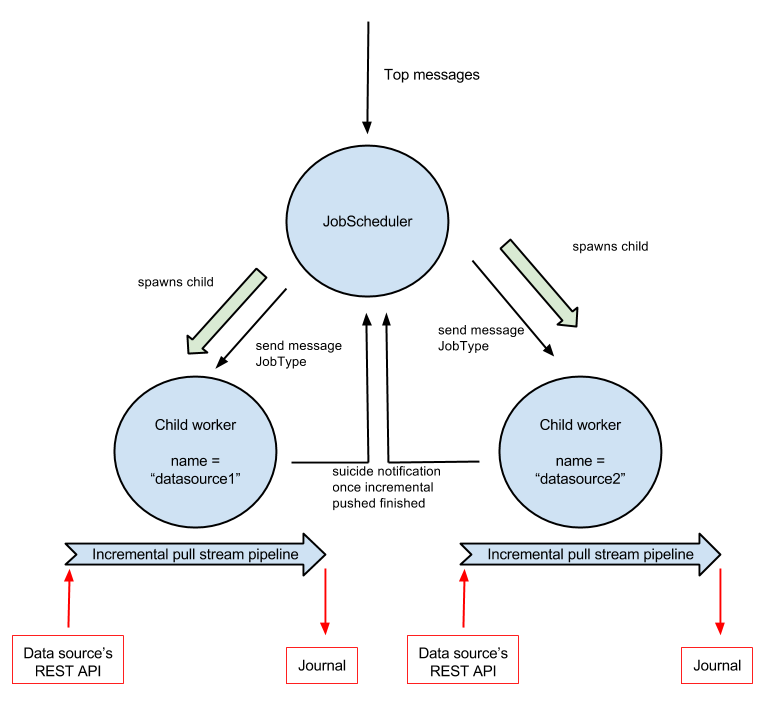
\includegraphics[width=1.0\textwidth]{img/archi_actor_dataintegration.png}}
    \caption{Puller actor system}
    \label{fig:archi_actor_dataintegration}
  \end{center}
\end{figure}

The JobScheduler must handle the fact that the job message rate for a data source can be faster than the incremental pull
of this data source (for example if the data source has produced a lot of new data since the last pull, or if it experiences some network problems). If a pull is still running when 
a new job message arrives for a data source, the JobScheduler should ignore the new pull message to avoid doing two or more pull in parallel of the same data source and risking a wrong
order of events. The JobScheduler can do this by assigning the name of the data source when it spawns a new worker child. Then, when a new job message comes in, it checks if it has a child of this name, and only if it has not it spawns a new child. 


\subsection{Incremental pull jobs}

When it is launched, each job must do an incremental pull on a particular data source via its REST API. For each the data source that the platform must integrate, there exists
a GET method that allows to get all the resource ids that were updated in a descendant order. The GET response is paginated, meaning that ids are coming 50 by 50 for example (the 
API caller has to make several call). 

Thus, a pull job has to pull the event ids that were updated after the last incremental pull. To do this, we define a stream where the producer makes one or several call to the
paginated REST API to produce a stream of JSON containing the ids of the resources updated. The producer must stop pulling when the date of the current update is less than the last
update event processed during the previous job. In order to persist for each job the date of the last event processed, we use a MongoDB database with a collection that stores a 
document with all the last event processed of each data source.

Moreover, for each resource, we are only interested in keeping the last update. Indeed, the REST API only gives us the type of update with the id of the resource, so if we pull (in desc order) a delete event before an update event, we want only to retain the delete event.

Then, the stream of events should be re-sorted in ascendant order, then for each event we must query the REST API to transform the resource id in the resource itself, then we must clean the resulting JSON to transform it to a known data model, then create an Journal event to insert in the Journal, and finally update MongoDB with the date of the last event.
Figure \ref{fig:pulljobpipeline} illustrates this pipeline in a simple schema. 

This stream pipeline must asynchronously process events while keeping ordering of messages, so Iteratees and Futures will be used to meet these requirements.
\\

Such an architecture allows transparent concurrency and parallelism up to the number of cores. Each child actor is executed concurrently, and the asynchronous stream processing
is using Iteratees that use Futures to allow transparent concurrency.

Moreover, the Actor model also allows easy distribution. In this architecture, the JobScheduler can transparently spawns some worker children in other machines. The implementation part
will detail this part more thoroughly.


\section{Implementation}










